
\chapter{\uppercase{Analysis}}

FIXME: regenerate all the graphs

Every user who has multiple contacts will have some contacts who are much
closer than others. In order to estimate the locations of users, we would like
to find out which users are most likely to live nearby.  In this section, we
investigate how various types of contacts correlate with proximity.
All of the analysis in this section was done on the contacts of FIXME \~250K users
with a home location.
Contacts with a PLE greater than or equal to 1000 miles were filtered out.

\section{What type of contact is closest?}

\begin{figure}[h]
\centering
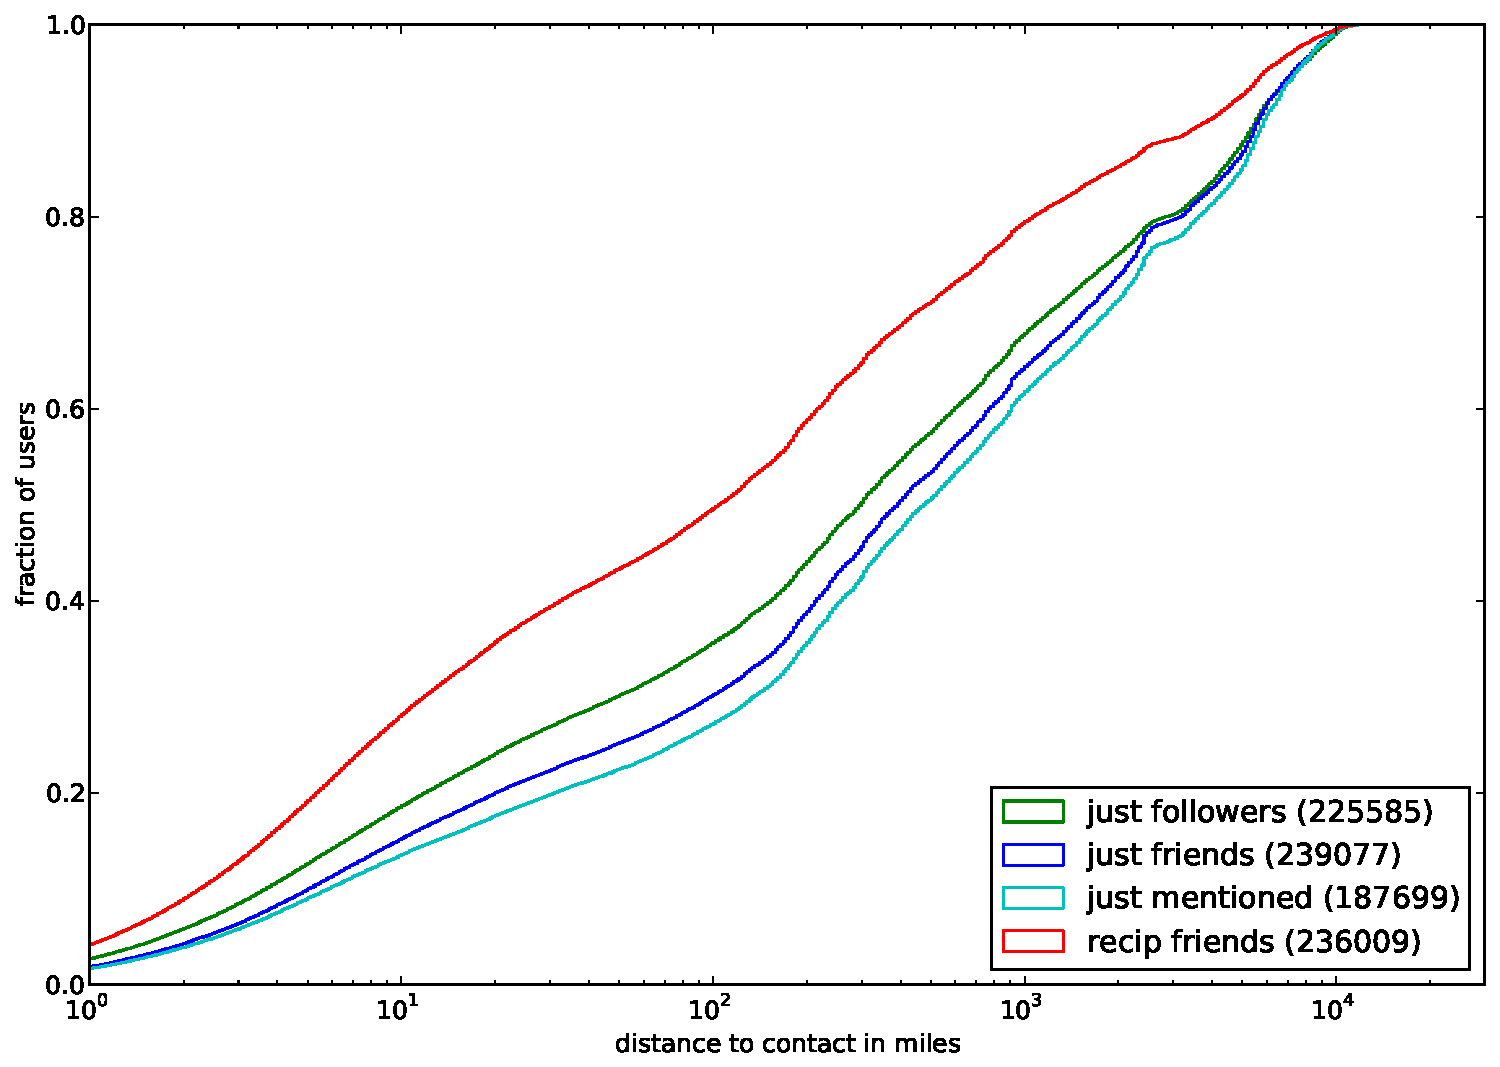
\includegraphics[width=\linewidth]{figures/edge_types_cuml.pdf}
\caption{
CDF of distance from geo-located users to users they have some contact
with.
The curves in this figure are the integrals of the curve in Figure \ref{fig:EdgeTypes}.
}
\label{fig:EdgeTypesCum}
\end{figure}

Figure~\ref{fig:EdgeTypesCum} shows the cumulative distribution
function(CDF) of the distance between a geo-located user and several types of
contacts.
Distance is plotted on a logarithmic scale to show both local and
global effects.

In general, reciprocal friends are the closest, followed by followers, friends,
and finally users who are just mentioned.
FIXME\% of reciprocal friends live within 25 miles while only FIXME\% of users
who are just mentioned live within that radius.
While it may seem that since being followed by someone and following someone
should be identical, they are not.
Celebrity and news accounts on Twitter often have large numbers of followers,
but they normally do not follow a large number of users.
Since the geo-located user was selected randomly, they are usually an average
user and not a celebrity.
If they follow someone, it might be a celebrity; however, if someone follows
them, it is probably someone who knows them.

FIXME: generalize this
There is a strange corner in the top right corner of all the graphs at
approximately 2500-2750 miles.
This is caused by the large population living on the coast, and the minuscule
number of people posting tweets from the Atlantic and Pacific oceans.

\section{What is the distribution of contacts?}

\begin{figure}[h]
\centering
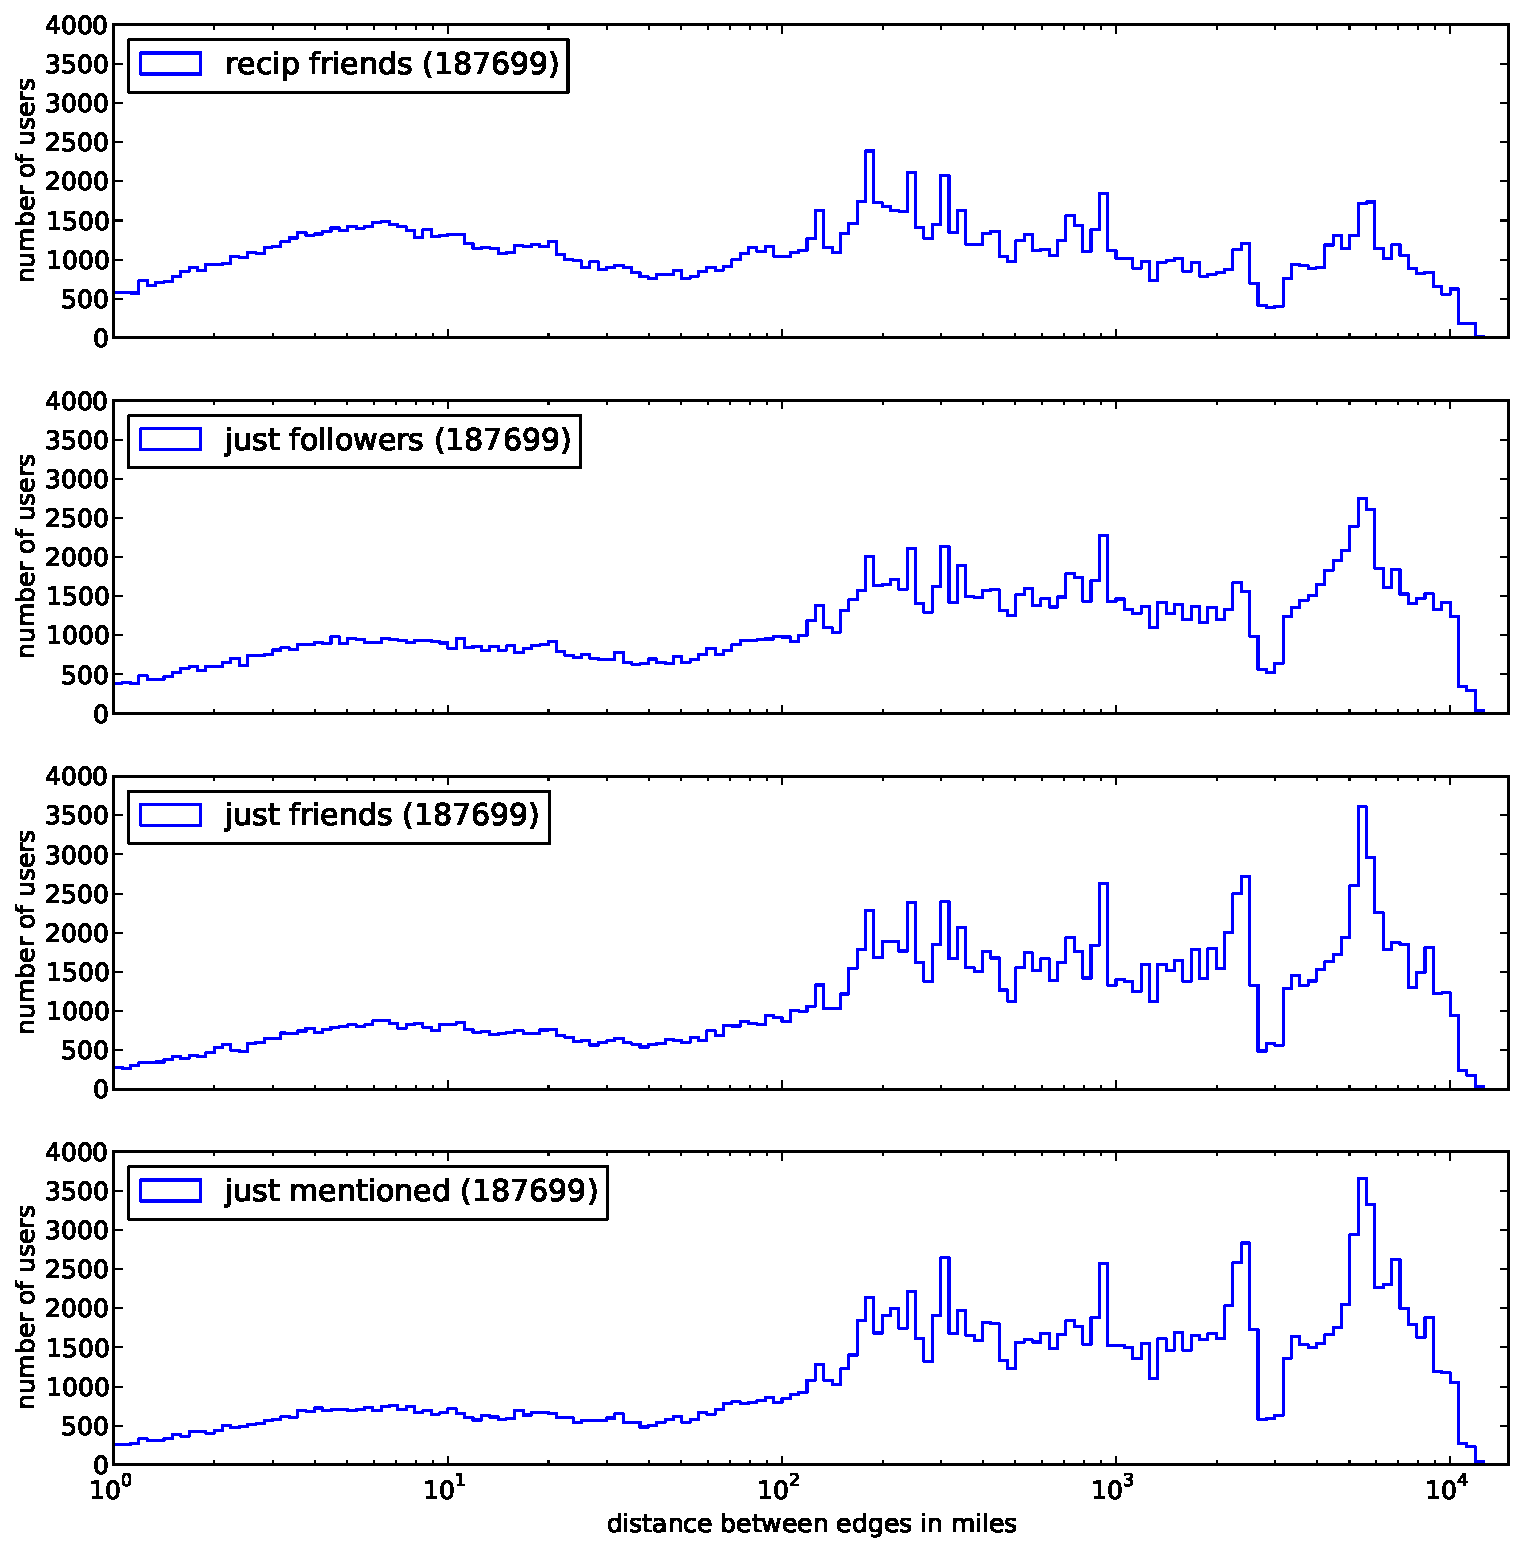
\includegraphics[width=\linewidth]{figures/edge_types_norm.pdf}
\caption{
Smoothed histogram of distance to users for different types of relationships.
%The dotted black line was created by calculating the distance between random, unrelated users.
}
\label{fig:EdgeTypes}
\end{figure}

To understand the distribution of contacts, we created a smoothed histogram.
First, the distances between contacts are sorted into 200 logarithmically
scaled bins (40 bins for each power of 10). Next, the curve is smoothed by
convoluting it with a seven element triangular window.
Figure~\ref{fig:EdgeTypes} (on FIXME) shows the result of plotting the
smoothed histogram.
All four types of contacts follow roughly the same bimodal
distribution: one peak around 10 miles from people who live nearby, and another
peak around 2500 miles, which is approximately the distance from coast to
coast.

FIXME: do we still want to look at the random friends
The geo-located users and their reciprocal friends were shuffled so that they
would be paired with someone who was probably not their friend and then
calculated the distance between the pair.
The dotted black line shows the results of this procedure.
For distances greater than around five
hundred miles, the red line and the black line have roughly the same shape,
which suggests that people when people are far away, their physical location no
longer matters.
The random line also has a similar shape to the other curves for distances
greater than 100 miles.

FIXME: bimodal has changed.
One reasonable explanation for this is that Twitter is not just a social
network; it is also a news distribution network.  This bimodal distribution
suggests that users have two types of contacts: people who they met in
real life, and people who they met online or know about via mainstream media.
The former group is useful for predicting location and the latter group is not.
In section~\ref{sec:model}, we use this idea that there are two types of
contacts to build a predictive location model based on social ties.


\section{Are users closer to people they communicate with?}

\begin{figure}[h]
\centering
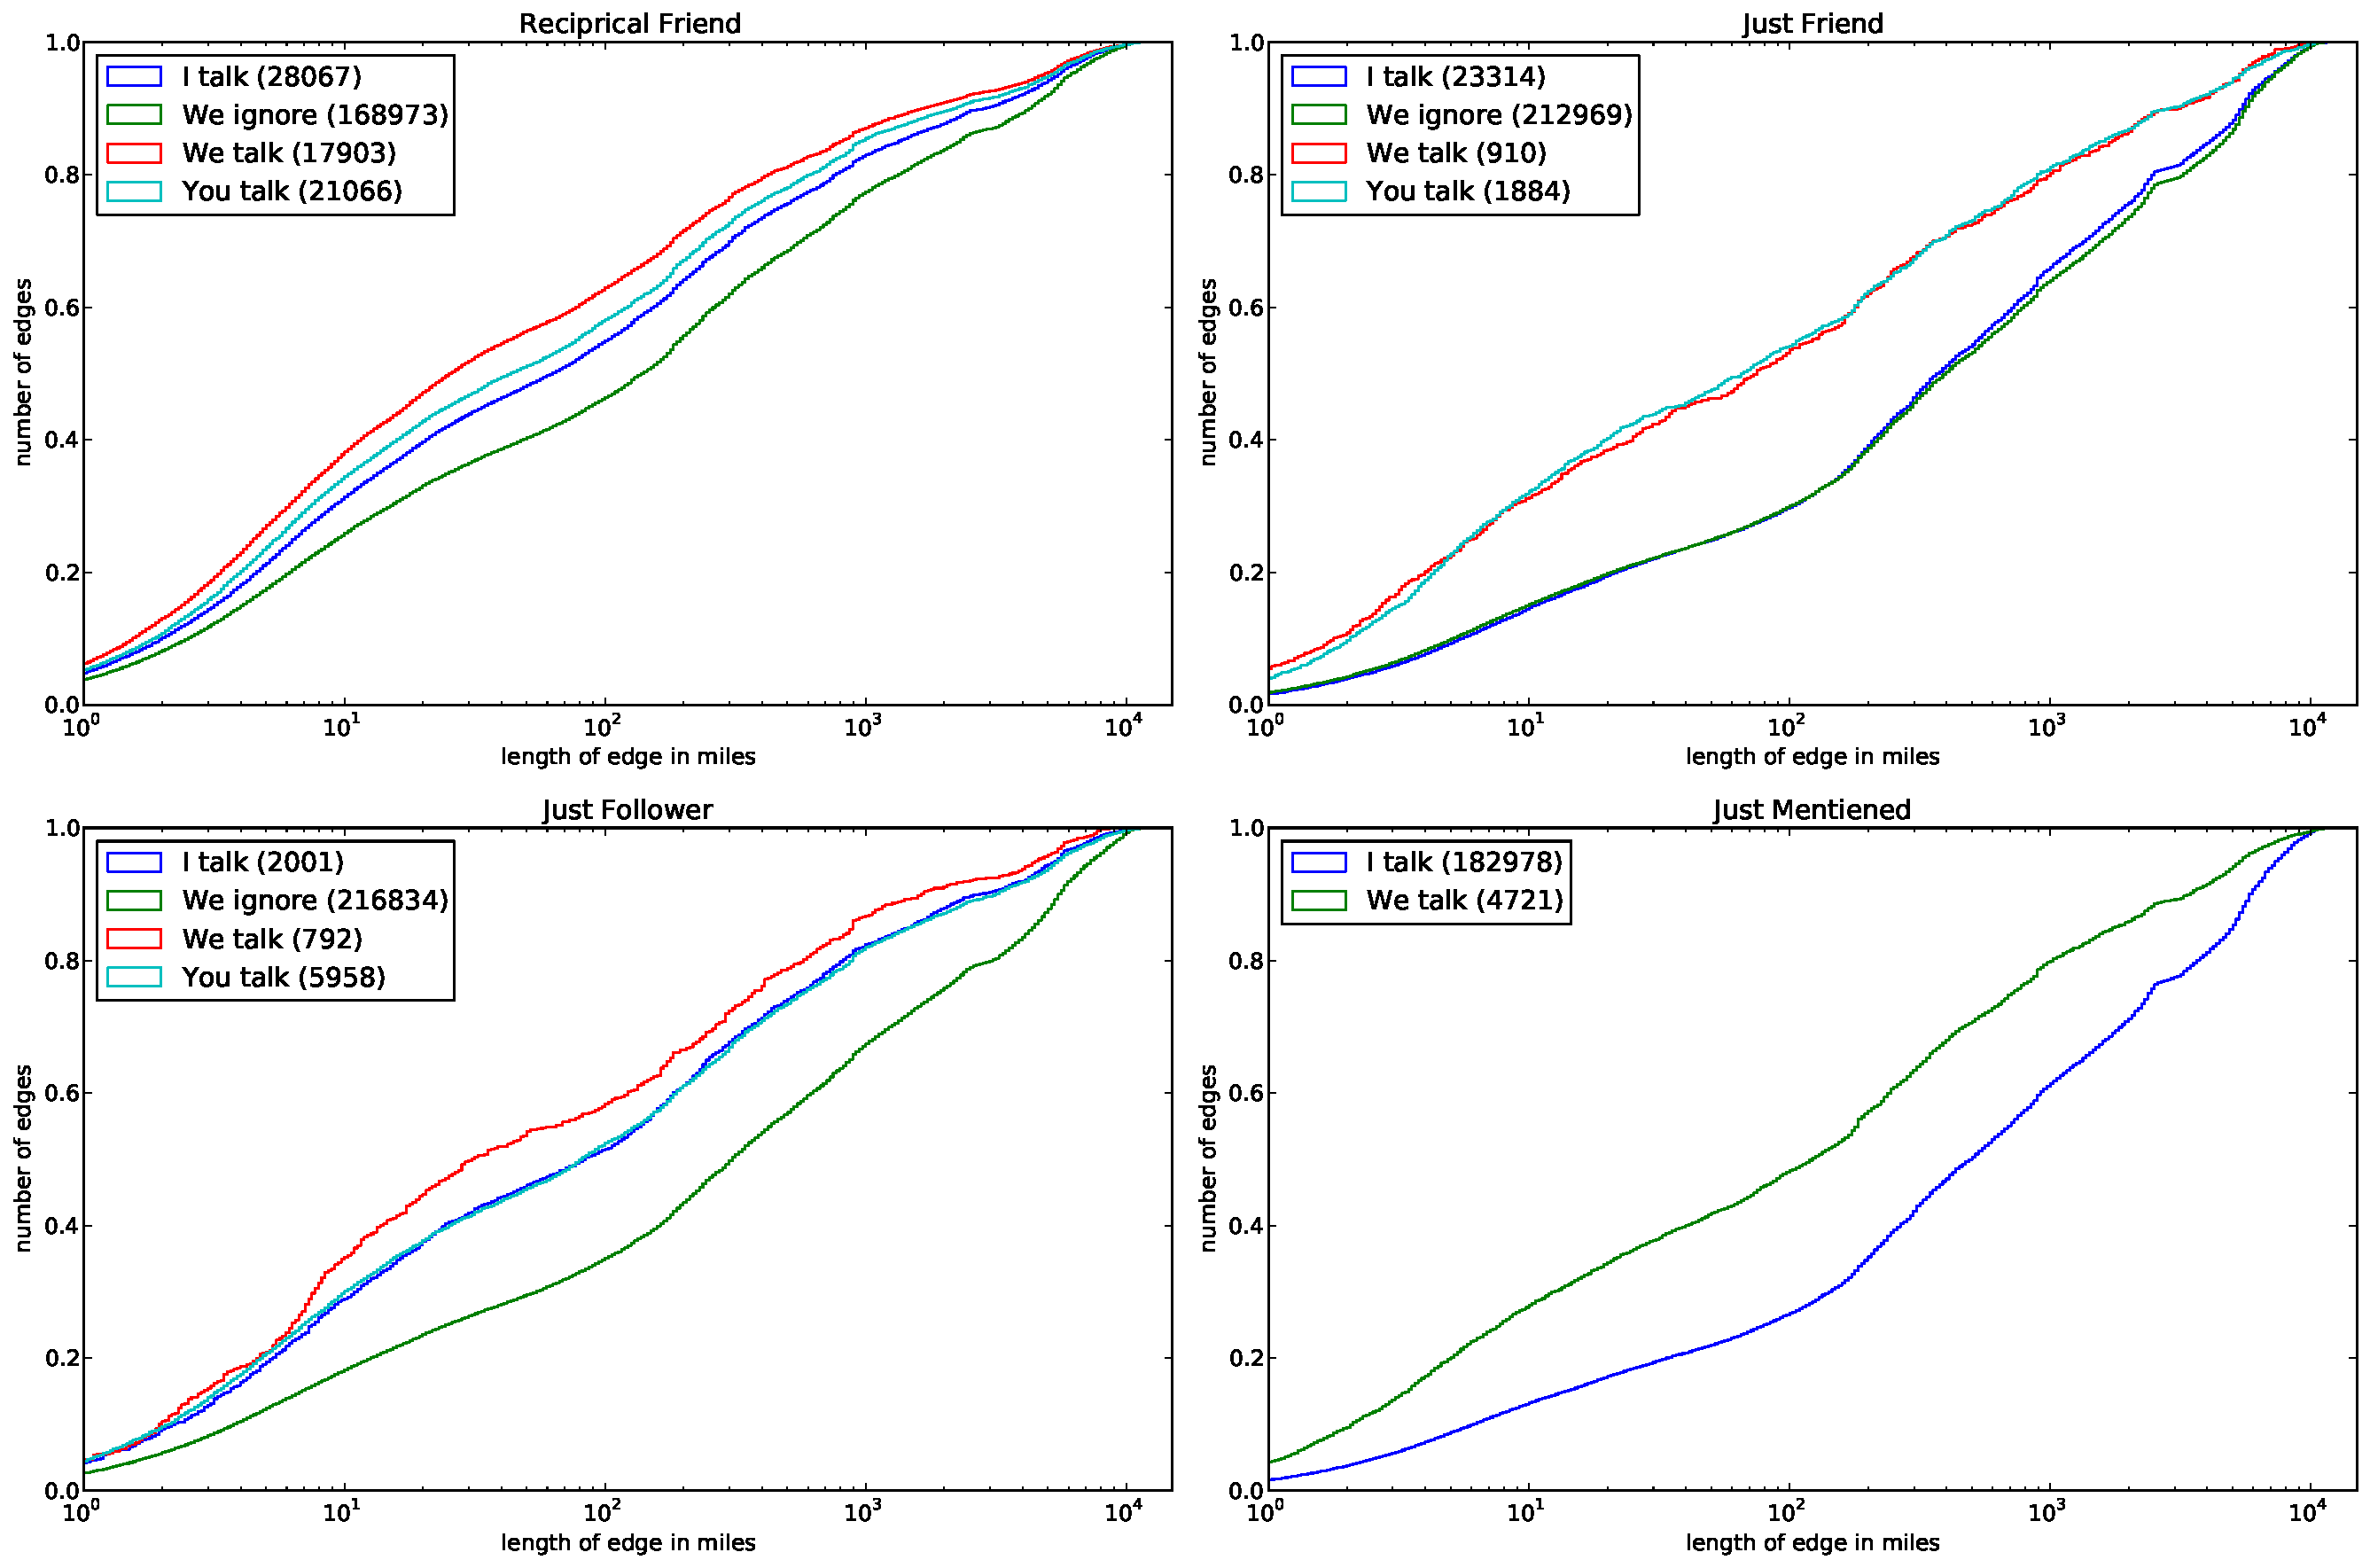
\includegraphics[width=\linewidth]{figures/com_types.pdf}
\caption{
CDF of the distance between a geo-located user and various types of contacts piloted on a logarithmic scale.
In these graphs, ``I'' refers to the geo-located user. ``You'' refers to their contact.
}
\label{fig:ComTypes}
\end{figure}

Figure~\ref{fig:ComTypes} shows the relationship between various types of
communication patterns between the geo-located users and their contacts.
Each of the four graphs visualize the same number of edges on the social graph
with the exception of the Just Mentioned graph. Approximately FIXME? one-third of our
geo-located users never mentioned someone who was not a friend or a follower,
so the sample size is smaller.

In almost every case, increased communication increases the probability that
two users live near each other.
There is one exception: when an average user mentions someone they follow who
does not follow them back, it has no effect.
In other words, if a random user mentions a celebrity who does not bother to
reply, they probably do not live in the same area. This can be seen by the blue
and green lines that are right on top of each other in the Just Friend graph.
On the other hand, in the rare event that someone who is just a friend replies
to their follower, then the probability that they live near each other is much
higher.

The weakest type of contact is for users who were just mentioned, but never
replied to, but if the person is mentioned, then FIXME\% of users with no
friend/follow relationship who have a conversation live within 25 miles.
This is approximately equal to the FIXME\% of reciprocal friends who ignore each
other and live within 25 miles.
Unsurprisingly, the strongest type of connection is reciprocal friends who
communicate.


\section{Are users closer to private accounts?}

\begin{figure}[h]
\centering
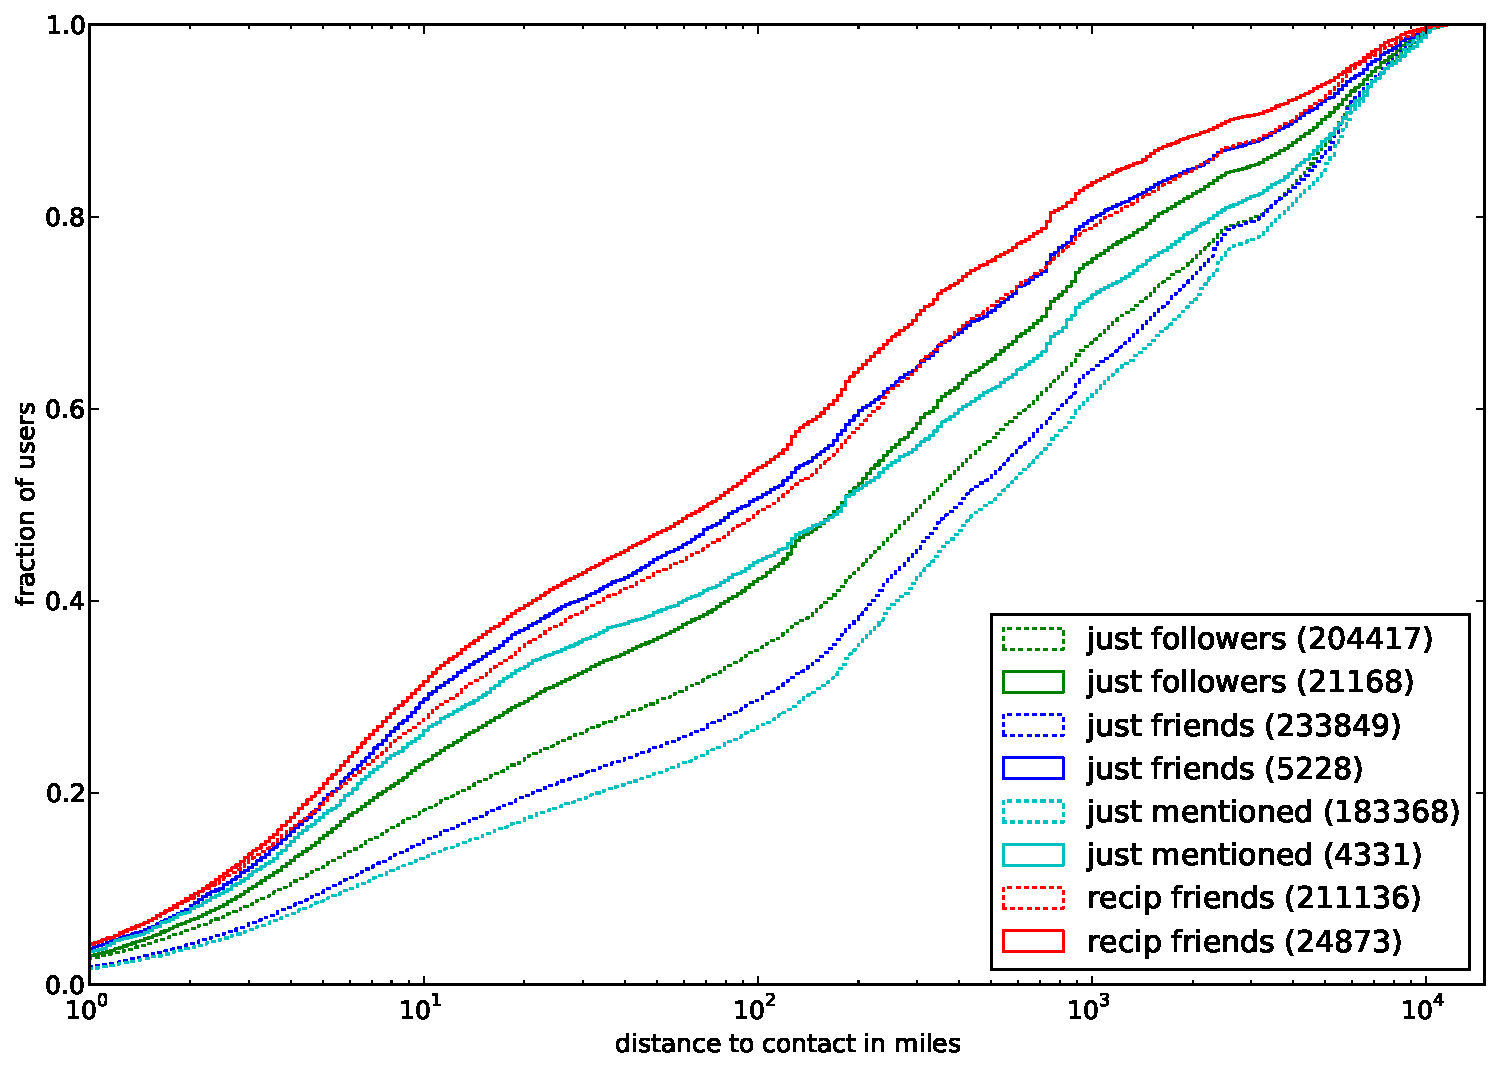
\includegraphics[width=\linewidth]{figures/edge_types_prot.pdf}
\caption{Solid lines represent protected accounts, and dashed lines represent public accounts. If a user follows a protected account, they tend to be closer.}
\label{fig:EdgeTypesProt}
\end{figure}

Like many social networks, Twitter allows users to mark their account as
protected. The specifics differ from network to network, but in Twitter's case
a user has to be approved to follow a protected user.
There are demographic differences between public and protected accounts.
For example, Gilbert \cite{gilbert2008network} demonstrates that rural users
are more likely to make their accounts private than public accounts.
In the case of protected accounts on Twitter, basic information
about their profile such as their location and the number of friends and
followers is public, but their friends list, followers list, and the text of
their tweets is private, and not available for analysis.

The most dramatic difference between private and public occurs if a user
follows a protected account.
Since users generally only allow people they know to follow a protected
account, this brings the users almost as close together as if they were
reciprocal friends.
On the other hand, if a protected account follows the geo-located user, this is
almost insignificant.
FIXME: what exactly is insignificant?
FIXME reference the graph

\section{If two of your friends live near each other, does that increase the
chance that they live near you?}
In this section, we turn our attention to triangles of users.
Finding useful relationships between the edges of a social triangle is tricky
because the three distances depend on each other.
Unfortunately, it is fairly simple to show using the triangle inequality theorem
that if two users are 1000 miles apart, then the third member of the triangle
has to be at least 500 miles from one of the other two.
Since this isn't a useful result, we designed a more complex experiment to
analyze the relationship between the sides of the triangle.
A script searched for a specific pattern in the social network of the
reciprocal friends.  It needed four users who fit the following criteria:
\begin{itemize}
\item ``me'' is the geo-located user
\item ``you'' is reciprocal friends with ``me''
\item ``my'' has no relationship with ``you'' and is reciprocal friends with ``me''
\item ``our'' is reciprocal friends with both ``me'' and ``you''
\end{itemize}

It found this pattern in FIXME of the users in the training set.
If a user had multiple instances of this pattern, it picked one of them
randomly so that particular users would not bias the results.
Since our crawler only retrieved friend and follower information for at most
seven reciprocal friends per user, it is reasonable to assume that this pattern
is much more common, but the sample is more than enough data to draw some
conclusions.

Figure~\ref{fig:NearTriads} shows a comparison between the ``my'' users and the
``our'' users.
For each of the ``my'' users and the ``our'' users, we put them into one of
four logarithmically scaled bins based on their distance from the ``you'' user.
Then we plot the CDF for the distance to ``me'' for each user in the set. This
allows us to investigate the effect of mutual friendship on distance.
We report one very simple result: if two of your friends are close (within 10
miles), then whether they know each other or not is strongly affects how close
you are to them. If they are farther apart, it doesn't matter.
%
%\section{Does the type of triangle matter?}
%
%FIXME: do we even want to look at triangle type? I spent a lot of time on it,
%but it is strongly correlated with number of followers.
%
%In the previous section we looked at the relationships between groups of
%reciprocal friends.
%In this section, we will look at the various types of triangles where at least
%one of the six possible directed edges is missing.
%For the geo-located users and their contacts, our crawler stored the user ids
%for up to 5000 of their friends and followers.
%As a result, a script can detect these triangles by looking at user ids even if
%it knows nothing about the third user in the set.
%
%For the geo-located user and his contact, we look at four types of triangles:
%\begin{description}
%\item[star] Both users follow someone. (This person is probably a star.)
%\item[fan] Someone follows both users. (This person is a fan of both users.)
%\item[path] The geo-located user follows someone who follows the contact.
%\item[loop] The contact follows someone who follows the geo-located user.
%\end{description}
%
%For each of the users and their four types of contacts, a script examined their
%friend and follower lists to find these triangles.
%It filtered out triangles where both sides are reciprocal friends, since these
%are relatively common, and were investigated in the previous section.
%Since the number of users who have the types of triangles is about the same
%magnitude as the number of users who do not have it, we investigate the
%presence or absence of each of the four triangle types rather than the number
%of triangles or the ratio of one type of triangle to another.
%
%Figure~\ref{fig:TriadTypes} shows the CDF for each of these types of triangles
%for each of the four kinds of contacts.
%The solid lines represent triangles that do exist for the edge, and the dotted
%lines represent edges that do not exist.
%These triangles are not useful for discriminating between near and far users in
%the reciprocal friend case, but they are more useful for other types of
%friendships.
%The prescience or absence of the triangles is the most significant for the just
%mentioned and just friend cases.
%In general, the star case is the most common type of triangle, and it is also
%the least useful.
%This is particularly true in the just friends case where the CDF of contacts
%with the star pattern and those without it are rather close together.

\section{Does the number of friends and followers a person have affect how
close they are?}

FIXME: this is important: should we move it up?
FIXME: the LocalAll graph was too clever

Since the primary goal of this research is to predict the location of users, we
focus our attention on the number of friends and followers a contact has rather
than the counts for the geo-located user.
Users are split into bins based on their number of friends or followers.
We choose to split the bins at 4, 16, 64, 256, 1024, and 4096 because powers
of two made the bins too small, and as a result, too noisy.
This is used to create a histogram where the height of the bin represents the
fraction of users who live within 25 miles, and the width of the bin is the
number of users in the bin.
Figure~\ref{fig:LocalAll} shows the result of this procedure.
In each graph, the red area must be equal to the blue area since the same set
of users was used to create each of them.

In general, people who are more promiscuous followers and friends are less
likely to live nearby. This makes sense because it is easy to meet 5 Twitter
users in real life, but very few people know 500 twitter users who live in the
same town.

Mainstream media and celebrity accounts such as the New York Times and Lady
Gaga have millions of followers while normal users rarely have more than a few
hundred.
Follower count is a good way to distinguish celebrity and news accounts which
are useless for location prediction.
For example, if a just friend contact has fewer than or equal to 64 followers,
there is almost a fifty percent chance that the users live within 25 miles. On
the other hand, if the just friend contact has more than 4096 followers, then
there is less than a ten percent chance that they live within 25 miles.


\section{Do some people have mostly nearby friends and other people have mostly
distant friends?}
FIXME: yes!
FIXME: generate a graph for this

